\documentclass{standalone}
%% Show/hide steps for standalone work — edit this line:
\makeatletter\AtBeginDocument{\@buildstepset{1,2,3}}\makeatother
\usepackage{hsbcommon}
\usepackage{tikz}
\usepackage{amsmath}
\usepackage{eurosym}
% \usepackage{zxjatype}
% \usepackage[ipa]{zxjafont}
\usetikzlibrary{intersections, calc}
\usepackage{hsbcommon}
\begin{document}
    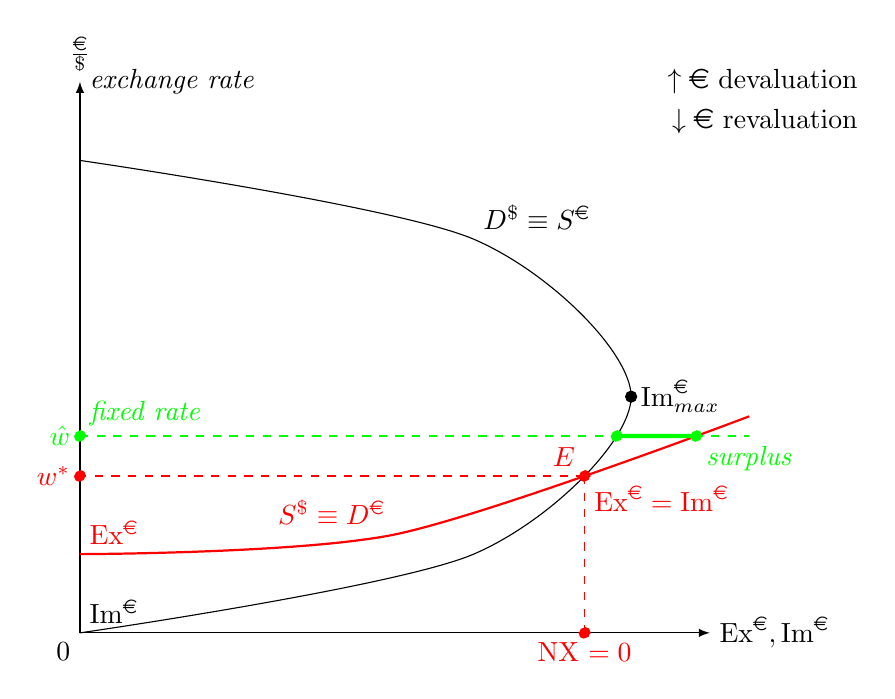
\begin{tikzpicture}
        \draw[->,>=latex] (0,0) node [below left] {0} -- (8,0) node[right] (w) {$\text{Ex}^\text{\euro} , \text{Im}^\text{\euro} $};
        \draw[->,>=latex] (0,0) -- (0,7) node[above] (P) {$\frac{\text{\euro} }{\$}$} node[right] {\textit{exchange rate}};

        \node[anchor=east] at (10,7) {$\uparrow \text{\euro} $ devaluation }; 
        \node[anchor=east] at (10,6.5) {$\downarrow \text{\euro} $ revaluation }; 

    \begin{scope} % Demand for currency: Imports

        \coordinate (A) at (0,6);
        \coordinate (B) at (5,5);
        \coordinate (C) at (7,3);
        \coordinate (D) at (5,1);
        \coordinate (E) at (0,0);
 
        \draw [name path global=demand] plot [smooth] coordinates {(A) (B) (C) (D) (E)}; \node [above right]  at (B) {$D^\$\equiv S^\text{\euro} $}; 
        \node [above right] at (E) {Im$^\text{\euro}$};
        
        % \filldraw (A) circle (2pt); \node[left] at (A) {$w_1^\text{Im}$};
        \filldraw (C) circle (2pt); \node[right] at (C) {$\text{Im}^{\text{\euro}}_{max}$};
        
    \end{scope}

    \ifstep{2}{
    
    
    \begin{scope}[red] % Offer of currency: Exports

        \coordinate (H) at (0,1);
        \coordinate (I) at (4,1.25);
        \coordinate (J) at (8.5,2.75);
 
        \draw [name path global=supply, thick] plot [smooth] coordinates {(H) (I) (J)}; \node [above left] (S) at (I) {$S{^\$} \equiv D^\text{\euro} $};
        % \filldraw (H) circle (2pt); \node[left] at (H) {$w_1^\text{Ex}$}; 
        \node[above right] at (H) {Ex$^{\text{\euro}}$};

        \begin{scope}[dashed]
    
            \path [name intersections={of=demand and supply,by=X}];
    
            \filldraw (X) node[above left]{$E$} circle (2pt); \node [below right] at (X) {$\text{Ex}^\text{\euro} =\text{Im}^\text{\euro} $};
            \draw (X) -- (X |-, 0); \filldraw (X |-, 0) circle (2pt); \node[below] at (X |-, 0) {NX $ =  0 $};
            \draw (X) -- (0, |- X); \filldraw (0, |- X) circle (2pt); \node[left] at (0, |- X) {$w^*$}; 
            
        \end{scope}
    
    \end{scope}    

    %% Different case: blue
    
    % \begin{scope}[blue] % Offer of currency: Exports

    %     \coordinate (H2) at (0,3.5);
    %     \coordinate (I2) at (5,4);
    %     \coordinate (J2) at (7.5,5);
 
    %     \draw [name path global=supplyzwei] plot [smooth] coordinates {(H2) (I2) (J2)}; \node [right] (S) at (J2) {$S{^\$} \equiv D^\text{\euro} $};
    %     \filldraw (H2) circle (2pt); \node[left] at (H2) {$w_2^\text{Ex}$}; \node[below right] at (H2) {\textit{export value}};


        % \begin{scope}[dotted]
    
        %     \path [name intersections={of=demand and supplyzwei,by=Y}];
    
        %     \filldraw (Y) circle (2pt);
        %     \filldraw (Y |-, 0) circle (2pt);
        %     \draw (Y) -- (Y |-, 0); \node[above left] at (Y |-, 0) {$Q^\dag$};
        %     \draw (Y) -- (0, |- Y); \node[left] at (0, |- Y) {$w^\dag$};
            
        % \end{scope}

    % \end{scope}

    }

    \ifstep{3}{
    
    \begin{scope}[green, dashed]
        \coordinate (Z) at (0,2.5); 
        \filldraw (Z) circle (2pt);
        \node[left] at (Z) {$\hat{w}$}; \node[above right] at (Z) {\textit{fixed rate}};
        \draw [name path=fixedrate] (Z) -- (8.5, |- Z);

        \path[name intersections={of=fixedrate and demand, by=Z1}];
        \path[name intersections={of=fixedrate and supply,by=Z2}];
        \filldraw (Z1) circle (2pt);
        \filldraw (Z2) circle (2pt); \node[below right] at (Z2) {\textit{surplus}};
        \draw[ultra thick,solid] (Z1) -- (Z2);
        
    \end{scope}
    }
    
    \end{tikzpicture}
\end{document}